% Inbuilt themes in beamer
\documentclass[aspectratio=169]{beamer}

\usepackage{listings}
\usepackage{inconsolata}
\usepackage{graphicx}
\usepackage{subcaption}
\usepackage{pifont}
\usepackage{wasysym}

\lstset{
  basicstyle=\ttfamily\footnotesize
}

\AtBeginSection[]{
  \begin{frame}
    \frametitle{Table of Contents}
    \tableofcontents[currentsection]
  \end{frame}
}

% Theme choice:
\usetheme{Frankfurt}

% Font choice:
\usefonttheme{serif}

% Title page details:
\title{MCNP Utilities: A Toolset for MCNP}
\author{Zack Dodson}
\date{}

\newcommand*{\vimage}[1]{\vcenter{\hbox{\includegraphics[width=0.24\textwidth]{#1}}}}
\newcommand*{\vpointer}{\vcenter{\hbox{\scalebox{2}{\Huge\pointer}}}}


\setbeamertemplate{footline}[frame number]
\setbeamertemplate{items}{\ding{227}}
\beamertemplatenavigationsymbolsempty

\begin{document}

% Title page frame
\begin{frame}
  \titlepage
\end{frame}

\section{Overview}

\begin{frame}{Overview}
  \begin{itemize}
    \item{
      MCNP Utilities: a toolset to assist with
      \begin{itemize}
        \item{\hyperlink{sec:input-file-generation}{Input file creation}}
        \item{\hyperlink{sec:post-processors}{Post-processing of output files}}
        \item{\hyperlink{sec:visualization}{Visualization of results}}
        \item{\hyperlink{sec:aux}{Other tasks}}
      \end{itemize}
    }
    \item{Includes re-written/modernized versions of tools that ship with MCNP (e.g., \lstinline{mattool}) or created by others (e.g., \lstinline{WORM})}
    \item{Some tools are very general, and some are very specific to a given use case}
    \item{
      All tools are command-line driven (works on all Windows and Unix-based machines)
      \begin{itemize}
        \item{Pass \lstinline{-h} to any tool for usage}
        \item{Repo contains a \lstinline{conda} environment file to help install all required modules}
        \item{Recommended: put the tools in your path so they can be called from anywhere}
      \end{itemize}
    }
  \end{itemize}
\end{frame}

\section{Input File Generation}\label{sec:input-file-generation}

\begin{frame}{Input File Generation Tools (Summary)}
  \begin{table}
    \resizebox{\textwidth}{!}{
      \begin{tabular}{l|l}
        \textbf{Tool}                                       & \textbf{Description}                                                             \\ \hline
        \hyperlink{compute-tmp}{\lstinline{compute_tmp.py}} & Convert temperature (any unit) to MeV for use in \lstinline{TMP} entry           \\ \hline
        \hyperlink{dose-scalar}{\lstinline{dose_scalar.py}} & Compute tally multiplier to convert scalar flux to dose (ACRR-specific)          \\ \hline
        \hyperlink{iso}{\lstinline{iso.py}}                 & Generate material card for any material mixture (rewrite of \lstinline{mattool}) \\ \hline
        \hyperlink{steadystate}{\lstinline{steadystate.py}} & k$_{\mathrm{eff}}$ or reactivity search tool                                                           \\ \hline
        \hyperlink{snake}{\lstinline{snake.py}}             & Create file permutations (rewrite of \lstinline{WORM})                 \\
      \end{tabular}
    }
  \end{table}
\end{frame}

\begin{frame}{Compute Cell Temperature}{\lstinline{utils/compute_tmp.py}}\label{compute-tmp}
  \begin{itemize}
    \item{Input temperature value and unit to get value in MeV}
    \item{Available units: \lstinline{C} (Celsius), \lstinline{K} (Kelvin), \lstinline{F} (Fahrenheit), or \lstinline{R} (Rankine)}
  \end{itemize}
  \begin{example}[1200$^{\circ}$C]
    \lstinputlisting{listings/compute_tmp_ex}
  \end{example}
\end{frame}

\begin{frame}{Compute Dose Scalar (per reactor energy yield)}{\lstinline{utils/dose_scalar.py}}\label{dose-scalar}
  \begin{itemize}
    \item{Input composition specification (same as \hyperlink{iso}{\lstinline{iso.py}})}
    \item{
      Provides the necessary tally scalar to compute dose in the material
      \begin{itemize}
        \item{\textbf{Use only for \lstinline{F4} tallies}}
        \item{\textbf{Assumes ACRR $\bar{\nu}$ and $\bar{Q}$}}
      \end{itemize}
    }
  \end{itemize}
  \begin{example}[Dose in Water]
    \lstinputlisting{listings/dose_scalar_ex}
  \end{example}
\end{frame}

\begin{frame}{Isotopic Structure Organizer (ISO) (1/3) -- Overview}{\lstinline{utils/iso.py}}\label{iso}
  \begin{itemize}
    \item{Rewrite (and extension) of \lstinline{mattool}}
    \item{Material analyzer \& card generator}
    \item{Can split elements into isotopic constituents}
    \item{
      Elements or isotopes can be specified via ZAID, name, or symbol
      \begin{itemize}
        \item{\lstinline{92235}}
        \item{\lstinline{Uranium-235}}
        \item{\lstinline{U-235}}
      \end{itemize}
    }
    \item{Can mix materials based on atom or weight fraction}
    \item{Can enrich materials with a specific isotope}
    \item{Can provide formatted material card and mixture molar mass (per atom)}
  \end{itemize}
\end{frame}

\begin{frame}{Isotopic Structure Organizer (ISO) (2/2) -- Ex. 1}{\lstinline{utils/iso.py}}
  \begin{example}[Water]
    \lstinputlisting{listings/iso_ex_1}
  \end{example}
\end{frame}

\begin{frame}{Isotopic Structure Organizer (ISO) (3/3) -- Ex. 2}{\lstinline{utils/iso.py}}
  \begin{example}[20 wt.\% UO$_2$ solution in water, 5 wt.\% enriched U]
    \lstinputlisting{listings/iso_ex_2}
  \end{example}
\end{frame}

\begin{frame}{Steadystate (Eigenvalue Search Tool)}{\lstinline{utils/steadystate.py}}\label{steadystate}
  \begin{itemize}
    \item{Can perform single-parameter k$_{\mathrm{eff}}$ or reactivity searches}
    \item{Can perform bisection search (and other types)}
    \item{Stops when search parameter is within specified tolerance (pcm or dollars)}
  \end{itemize}
  \begin{example}[k$_{\mathrm{eff}}$ Search for 1.0 with 50 pcm tolerance]
    \lstinputlisting{listings/steadystate_ex_1}
  \end{example}
  \begin{example}[Reactivity Search for 0\$ with 2 cents tolerance]
    \lstinputlisting{listings/steadystate_ex_2}
  \end{example}
\end{frame}

\begin{frame}{Snake (Python rewrite of \lstinline{WORM}) (1/3) -- Overview}{\lstinline{utils/snake.py}}\label{snake}
  \begin{itemize}
    \item{Scriptable Nesting and Keying Engine (SNAKE)}
    \item{Creates permutations of a file based on specified keys in an input file}
    \item{Expressions that define variables (constants or keys) are contained in curly braces}
    \item{Allow usage of user-defined Python functions}
    \item{Python f-string syntax is used for printing variables}
    \item{
      Output files:
      \begin{itemize}
        \item{Named by key index (but naming by value can be specified)}
        \item{Can be organized into a hierarchical directory structure (optionally)}
        \item{File extension can be specified}
      \end{itemize}
    }

    \item{A key file can be created that contains a mapping of key values to file names}
  \end{itemize}
\end{frame}

\begin{frame}{Snake (Python rewrite of \lstinline{WORM}) (2/3) -- Ex. 1}{\lstinline{utils/snake.py}}
  \begin{block}{Snake Input File (\lstinline{case_1.snake})}
    \lstinputlisting{listings/case_1.snake}
  \end{block}
  \begin{example}
    \lstinputlisting{listings/snake_ex_1}
  \end{example}
\end{frame}

\begin{frame}{Snake (Python rewrite of \lstinline{WORM}) (3/3) -- Ex. 2}{\lstinline{utils/snake.py}}
  \begin{block}{Snake Input File (\lstinline{case_2.snake})}
    \lstinputlisting{listings/case_2.snake}
  \end{block}
  \begin{block}{\lstinline{my_fn.py}}
    \lstinputlisting[language=python]{listings/my_fn.py}
  \end{block}
  \begin{example}[User-Defined Function]
    \lstinputlisting{listings/snake_ex_2}
  \end{example}
\end{frame}

\section{Post-Processors}\label{sec:post-processors}

\begin{frame}{Post-Processor Tools (Summary)}
  \begin{table}
    \resizebox{\textwidth}{!}{
      \begin{tabular}{l|l}
        \textbf{Tool}                                                 & \textbf{Description}                                                    \\ \hline
        \hyperlink{get-rx}{\lstinline{get_rx.py}}                     & Determine reactivity (in dollars) of model from output file             \\ \hline
        \hyperlink{tallies}{\lstinline{tallies.py}}                   & Extract all tallies from output file into Python dictionary             \\ \hline
        \hyperlink{meshtal-to-h5}{\lstinline{meshtal_to_h5.py}}       & Convert ASCII mesh tally results to HDF5 for use with other tools       \\ \hline
        \hyperlink{extract-spectrum}{\lstinline{extract_spectrum.py}} & Extract spectra from MCNP output file for plotting                      \\
      \end{tabular}
    }
  \end{table}
\end{frame}

\begin{frame}{Reactivity Extractor}{\lstinline{utils/get_rx.py}}\label{get-rx}
  \begin{itemize}
    \item{Extracts reactivity from MCNP output file (must have \lstinline{KINETICS} enabled)}
    \item{Can process directories and extract data to Excel}
    \item{Can compute reactivity difference relative to specified file}
  \end{itemize}
  \begin{example}
    \lstinputlisting{listings/get_rx_ex}
  \end{example}
\end{frame}

\begin{frame}{Tally Extractor}{\lstinline{utils/tallies.py}}\label{tallies}
  \begin{itemize}
    \item{Extracts tallies from MCNP output file}
    \item{Organized by tally \#, cell \#, material \#, and then energy bin}
    \item{Provides the function \lstinline{get_all_tallies}, which returns a \lstinline{dict} with all tallies}
  \end{itemize}
  \begin{example}
    \lstinputlisting{listings/tallies_ex}
  \end{example}
\end{frame}

\begin{frame}{ASCII Mesh Tally to HDF5 Converter}{\lstinline{utils/meshtal_to_h5.py}}\label{meshtal-to-h5}
  \begin{itemize}
    \item{
      Converts legacy (ASCII) meshtal file to HDF5 format
      \begin{itemize}
        \item{Only works on ASCII-formatted meshtal files (\lstinline{OUT=COL|COLSCI}) (default thru MCNP 6.3.1)}
      \end{itemize}
    }
    \item{
      Allows usage with other tools in this module
      \begin{itemize}
        \item{\hyperlink{plot-meshtally}{\lstinline{plot_meshtal.py}}}
        \item{\hyperlink{paramesh}{\lstinline{paramesh.py}}}
      \end{itemize}
    }
    \item{Reduces file size}
  \end{itemize}
  \begin{example}
    \lstinputlisting{listings/meshtal_to_h5_ex}
  \end{example}
\end{frame}

\begin{frame}{Spectrum Extractor}{\lstinline{utils/extract_spectrum.py}}\label{extract-spectrum}
  \begin{itemize}
    \item{Extract spectrum data from MCNP output file for plotting with \hyperlink{plot-spectra}{\lstinline{plot_spectra.py}}}
  \end{itemize}
  \begin{example}
    \lstinputlisting{listings/extract_spectrum_ex}
  \end{example}
\end{frame}

\section{Visualization of Results}\label{sec:visualization}

\begin{frame}{Visualization Tools (Summary)}
  \begin{table}
    \resizebox{\textwidth}{!}{
      \begin{tabular}{l|l}
        \textbf{Tool}                                           & \textbf{Description}                              \\ \hline
        \hyperlink{cropper}{\lstinline{crop_mcnp_plot.py}}      & Crop MCNP-generated plots for publication         \\ \hline
        \hyperlink{plot-spectra}{\lstinline{plot_spectra.py}}   & Create energy-dependent neutron or gamma plots    \\ \hline
        \hyperlink{compute-pf}{\lstinline{compute_pf.py}}       & Create peaking factor plots                       \\ \hline
        \hyperlink{plot-meshtally}{\lstinline{plot_meshtal.py}} & Visualize mesh tally output                       \\ \hline
        \hyperlink{paramesh}{\lstinline{paramesh.py}}           & Convert mesh tally to vtu files (ParaView) \\
      \end{tabular}
    }
  \end{table}
\end{frame}

\begin{frame}{MCNP Plot Crop Tool}{\lstinline{utils/crop_mcnp_plot.py}}\label{cropper}
  \begin{itemize}
    \item{For MCNP geometry plots generated from the command line or saved using the plotter}
    \item{Crops the plot appropriately to remove extraneous information}
  \end{itemize}
  \begin{example}
    \lstinputlisting{listings/crop_mcnp_plot_ex}
  \end{example}
  \centering
  $\vimage{figs/ACRR-core-uc}\vpointer\vimage{figs/ACRR-core-c}$
\end{frame}

\begin{frame}{Spectral Plotter}{\lstinline{utils/plot_spectra.py}}\label{plot-spectra}
  \begin{itemize}
    \item{Plot multiple tally spectra (per lethargy for visual accuracy)}
    \item{Spectral data can be normalized}
    \item{1-$\sigma$ errorbars can be optionally included}
  \end{itemize}
  \begin{example}
    \lstinputlisting{listings/plot_spectra_ex}
  \end{example}
  \centering
  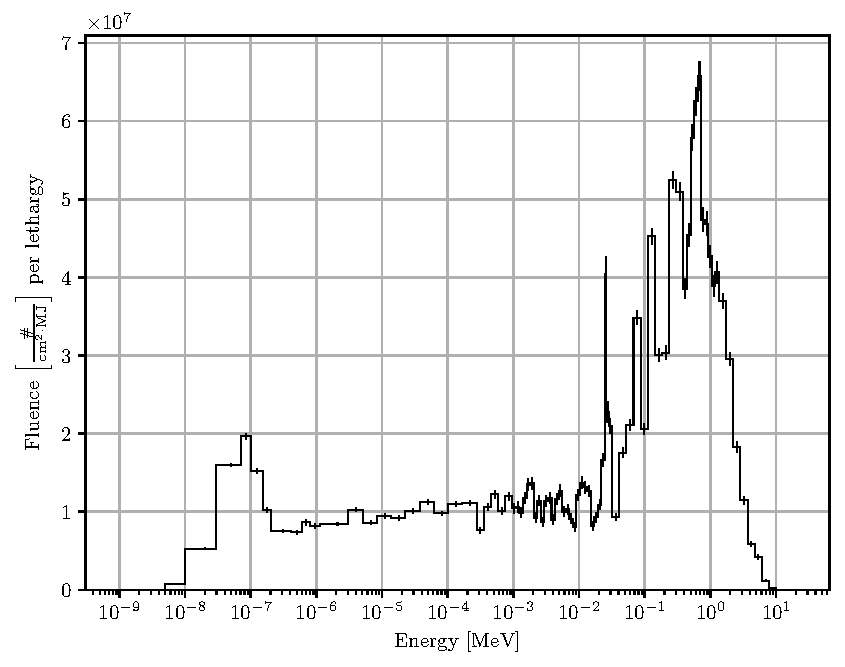
\includegraphics[width=0.32\textwidth]{figs/my_spec}
\end{frame}

\begin{frame}{Compute and Plot Peaking Factors}{\lstinline{utils/compute_pf.py}}\label{compute-pf}
  \begin{itemize}
    \item{Read lattice tallies from MCNP output to create peaking factor plots}
  \end{itemize}
  \begin{example}
    \lstinputlisting{listings/compute_pf_ex}
  \end{example}
  \centering
  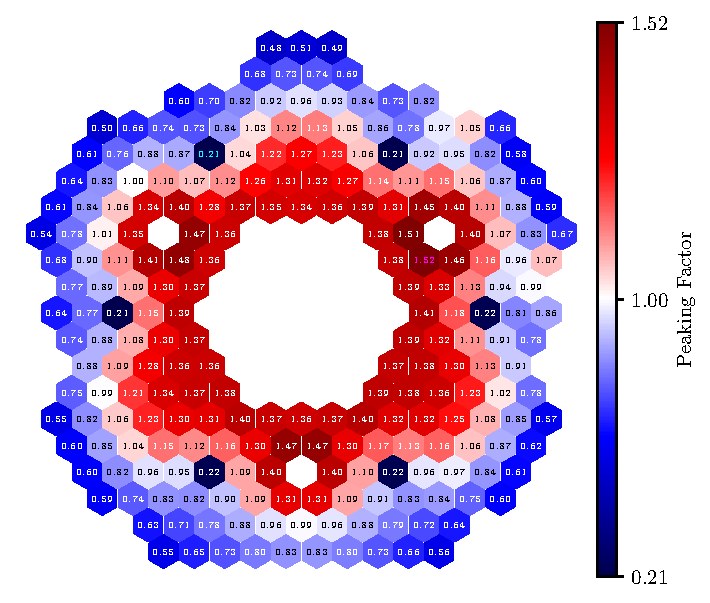
\includegraphics[width=0.34\textwidth]{figs/PF}
\end{frame}

\begin{frame}{Plot Mesh Tally (1/4) -- Overview}{\lstinline{utils/plot_meshtal.py}}\label{plot-meshtally}
  \begin{itemize}
    \item{Input tally \#, plot name, \lstinline{meshtal.h5} file (converted from ASCII) or \lstinline{runtpe.h5} file, and plot domain (1D [line] or 2D [plane])}
    \item{Data is summed over energy groups by default, but a specific group can be chosen}
    \item{Contour plots are also possible by defining the threshold values and colors}
    \item{Works for Cartesian and cylindrical geometry (not spherical)}
    \item{Can sum two datasets and properly propagate statistical error (via summation in quadrature)}
  \end{itemize}
\end{frame}

\begin{frame}{Plot Mesh Tally (2/4) -- 1D Plot}{\lstinline{utils/plot_meshtal.py}}
  \begin{example}
    \lstinputlisting{listings/plot_meshtal_ex_1D}
  \end{example}
  \centering
  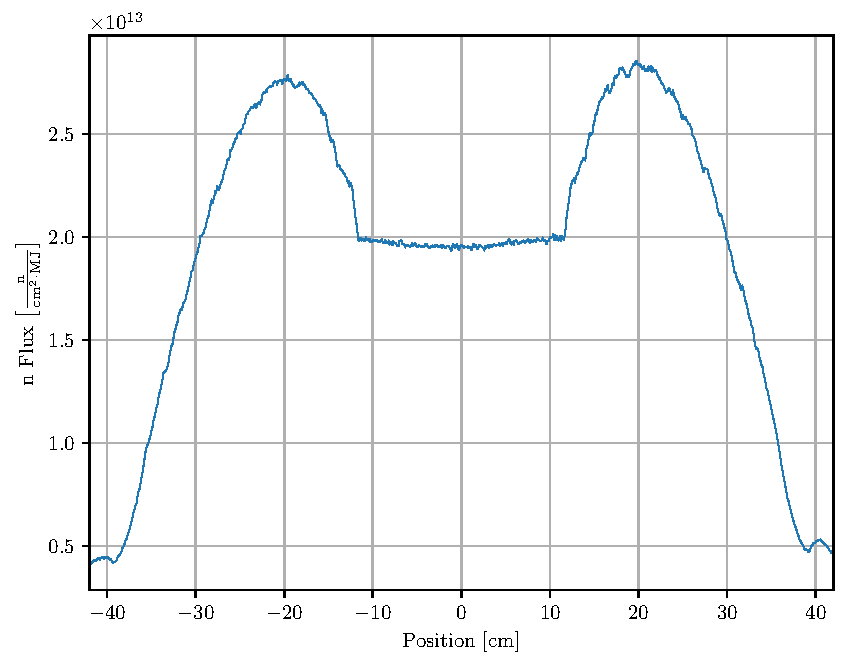
\includegraphics[width=0.39\textwidth]{figs/flux-1D}
\end{frame}

\begin{frame}{Plot Mesh Tally (3/4) -- 2D Plot}{\lstinline{utils/plot_meshtal.py}}
  \begin{example}
    \lstinputlisting{listings/plot_meshtal_ex_2D}
  \end{example}
  \centering
  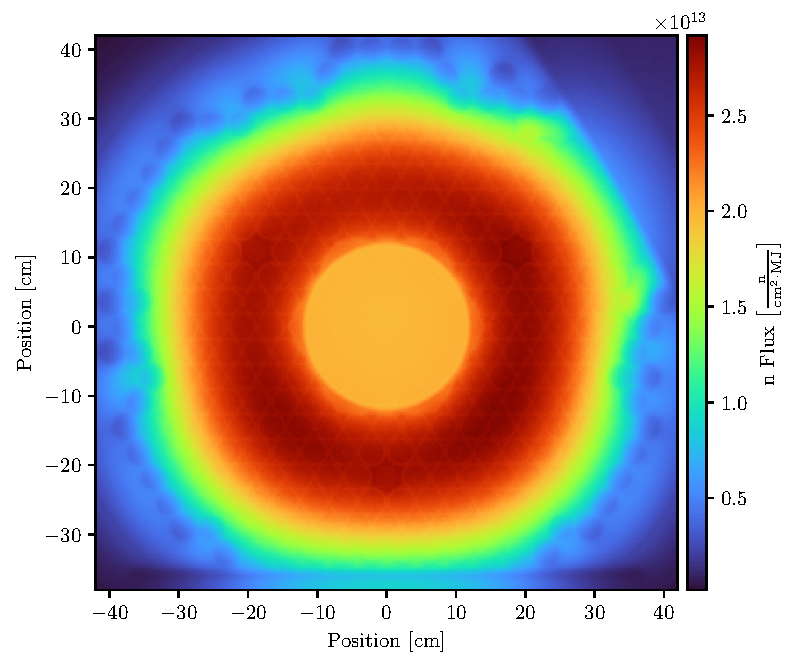
\includegraphics[width=0.37\textwidth]{figs/flux-2D}
\end{frame}

\begin{frame}{Plot Mesh Tally (4/4) -- Contour Plot}{\lstinline{utils/plot_meshtal.py}}
  \begin{example}
    \lstinputlisting{listings/plot_meshtal_ex_contour}
  \end{example}
  \centering
  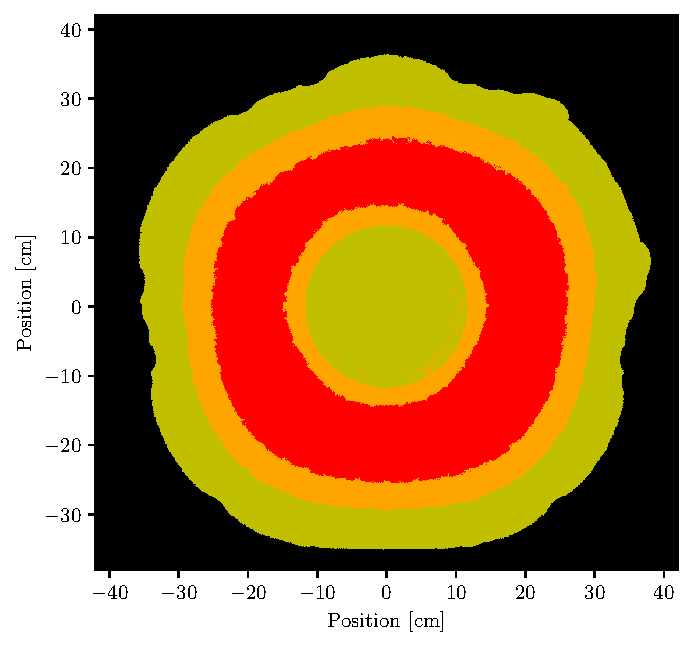
\includegraphics[width=0.36\textwidth]{figs/flux-c}
\end{frame}

\begin{frame}{Paramesh}{\lstinline{utils/paramesh.py}}\label{paramesh}
  \begin{itemize}
    \item{Convert mesh tally data to \lstinline{vtu} files that can be opened in ParaView}
    \item{Works on converted ASCII files or \lstinline{runtpe.h5} files with mesh tally data}
  \end{itemize}
  \begin{example}
    \lstinputlisting{listings/paramesh_ex}
  \end{example}
  \centering
  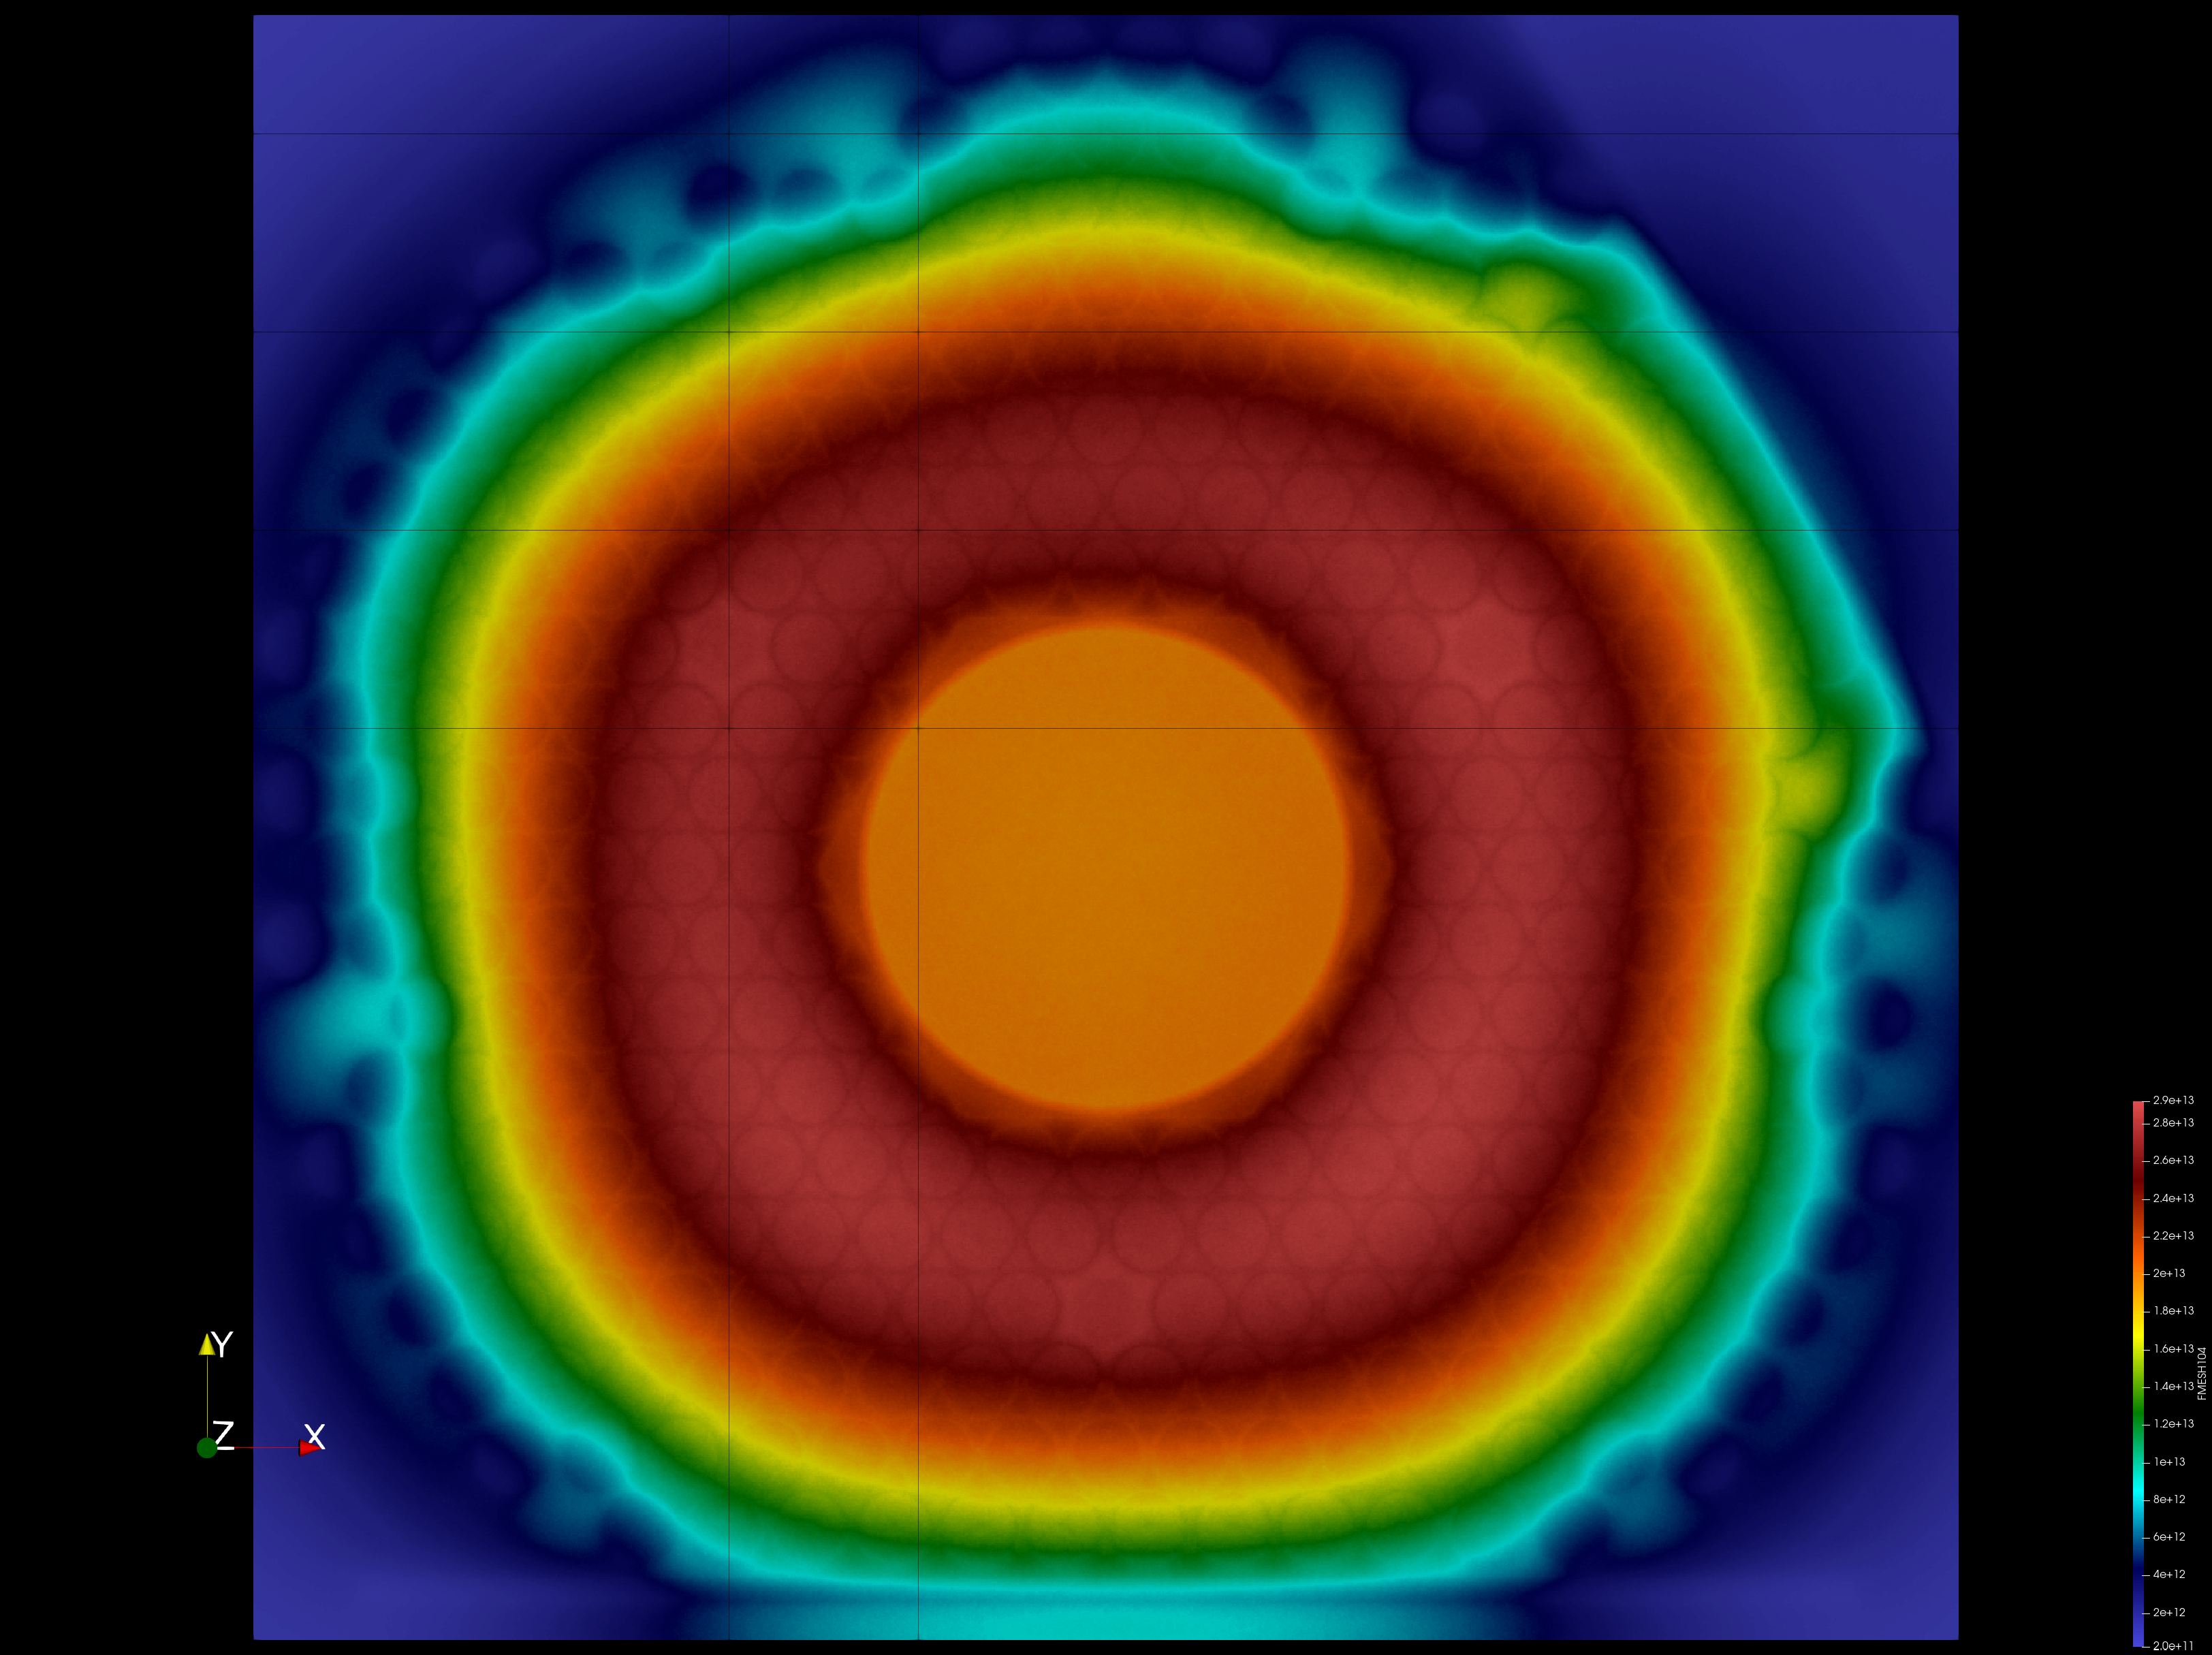
\includegraphics[width=0.37\textwidth]{figs/paraview}
\end{frame}

\section{Auxiliary Capability}\label{sec:aux}

\begin{frame}{\LaTeX\ Table Generator (1/2) -- Overview}{\lstinline{lib/tables.py}}
  \begin{itemize}
    \item{
      Generates \LaTeX\ table source code from Pandas/Polars DataFrame or dict
      \begin{itemize}
        \item{\lstinline{Pandas} has this capability but it is lacking}
      \end{itemize}
    }
    \item{Allows direct conversion of parsed/post-processed data to publication-quality table}
    \item{Supports \lstinline{table}, \lstinline{subtable}, and \lstinline{longtable}}
    \item{Numerous format options including numeric formatter functions}
  \end{itemize}
\end{frame}

\begin{frame}{\LaTeX\ Table Generator (2/2) -- Example}{\lstinline{lib/tables.py}}
  \vspace*{-1.2em}
  \begin{example}
    \lstinputlisting[basicstyle=\ttfamily\tiny,language=python]{listings/tables_ex.py}
  \end{example}
  \begin{block}{\lstinline{table.tex}}
    \lstinputlisting[basicstyle=\ttfamily\tiny]{listings/table.tex}
  \end{block}
  \vspace*{-6.8em}\hspace*{20em}
  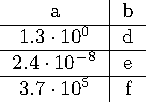
\includegraphics[width=0.2\textwidth]{listings/table.pdf}
\end{frame}

\begin{frame}
  \vfill
  \centering\Huge Questions?\\
  \vfill
\end{frame}

\end{document}
